\documentclass{article}

% ==========================================================================
% chi-VLA, NeurIPS 2026 VLM4RWD workshop submission
% Compile: pdflatex -interaction=nonstopmode chi-vla.tex  (twice)
% ==========================================================================

\PassOptionsToPackage{numbers,sort&compress}{natbib}
\usepackage[dblblindworkshop]{neurips_2026}
\workshoptitle{Grounded and Faithful Vision-Language Models for Real-World Deployment (VLM4RWD)}
\usepackage[utf8]{inputenc}
\usepackage[T1]{fontenc}
\usepackage{amsmath,amssymb,amsfonts}
\usepackage{booktabs}
\usepackage{graphicx}
\usepackage{xcolor}
\usepackage{tikz}
\usetikzlibrary{positioning,fit,backgrounds,arrows.meta}
\usepackage[colorlinks=true,linkcolor=blue,citecolor=blue,urlcolor=blue]{hyperref}
\usepackage{url}
\usepackage{float}
\usepackage{microtype}
\newcommand{\chivla}{$\chi$-VLA}
\newcommand{\R}{\mathbb{R}}

\title{\textbf{A Capable, Fully Tensor-Decomposable}\\[0.15em]
\textbf{Vision-Language-Action Policy}\\[0.35em]
\large Exact rational conversion, protocol-aligned control, and weight-derived causal structure}
\author{}
\date{}

\begin{document}
\maketitle

\begin{abstract}
Tensor decomposition factors a large table of interactions into a small set of low-rank
components that can be ranked and inspected. Applying it directly to a conventional robot
policy is difficult because softmax, ordinary activations, and normalization interrupt the
required algebraic form. We introduce \chivla, a compact vision-language-action policy whose
learned map uses only bilinear, linear, and rational operations. Its checkpoint therefore
defines an explicit rational tensor program, making interactions among image, instruction,
state, and action coordinates accessible from the weights. A mechanical audit finds no hidden
incompatible operation, and local reconstructions agree near the float32 precision floor.
On all ten LIBERO-Object tasks, the $20.1$M-parameter policy reaches $92.8\%\pm2.1\%$ with a
ViT encoder and $93.7\%\pm0.8\%$ with a convolutional encoder under the published three-seed
protocol. A same-skeleton conventional twin differs by only $0.006\%$ in parameters. An initial
mixed-device replication gives it $89.8\%$, versus $85.2\%$ for the rational checkpoint, so a
same-device capability matrix is required. Compilation reduces the same-A30 latency ratio from
$5.33\times$ in eager mode to $1.74\times$.
We derive an exact weight-based decomposition of softmax-free attention and reconstruct every
attention module in three checkpoints with worst relative error $2.56\times10^{-7}$. All $36$
primary block-head tests favor its rank-$128$ subspace over equal-rank random controls, with
median fidelity ratio $2.44$. At the policy's visual bond, retaining $64$ of $384$ causally
ranked dimensions preserves $18/20$ closed-loop successes, compared with $19/20$ for the full
representation and $0/20$ for a random subspace. A $300$-pair instruction intervention across
three checkpoints shows consistent language-driven motion but incomplete scene-prior override.
The evidence establishes competitive specialist capability and exact layerwise access, not a
settled architecture-level capability gap, broad generalization, compute parity,
or selective coefficient-level repair.
\end{abstract}

% ============================================================================
\section{Introduction}
% ============================================================================

Modern robot policies can work well while remaining difficult to inspect. A checkpoint contains
millions of learned numbers, but it does not directly reveal which combinations of image regions,
instruction tokens, and robot state produce an action. Analysts therefore usually collect
activations on a dataset and fit a separate probe. That can identify correlations, but it leaves
open whether the same structure is present in the weights and whether it causes behavior.

Tensor decomposition offers a different analysis surface. A tensor is a multidimensional table,
and a decomposition rewrites that table as a sum of simpler low-rank factors, much as a matrix
factorization finds dominant directions in a matrix. If a network is built from additions,
multiplications, and ratios of polynomials, its weights define an explicit table of input
interactions. Decomposing that table can rank the combinations the model is constructed to use.
By \emph{fully tensor-decomposable}, we mean that every learned block preserves this algebraic
form. The aim is not merely compression. It is a direct path from parameters to candidate
mechanisms that can be tested by intervention \cite{pearce,chinets}.

Robot control makes this goal useful and difficult. Visual shortcuts can produce high benchmark
success while ignoring the instruction, and small action errors compound in closed loop.
Standard softmax, nonlinear activations, and square-root normalization break the explicit
polynomial form. Continuous actions also cannot rely on the external categorical sampling used
by a language model. A practical design must recover these functions without losing precise
control.

We study the narrower but testable question:

\begin{quote}
\emph{Can a specialist VLA retain competitive closed-loop capability when every deployed
learned operation is polynomial or rational, and does the resulting structure provide a useful
weight-based analysis surface?}
\end{quote}

The stronger thesis has three parts: decomposability should have small capability cost, the
weights should expose stable behaviorally causal interactions, and editing those interactions
should selectively change behavior without retraining. This paper establishes strong capability
and exact layerwise structure, then states clearly where causal diagnosis and editing remain
incomplete.

Our contributions are:

\begin{enumerate}
  \item We construct a complete VLA from tensor-compatible primitives. A rational normalization
        supplies input-specific scaling without leaving the rational function class.
  \item We evaluate two fully rational $20.1$M-parameter policies under a protocol aligned with
        published LIBERO-Object results. The strongest single architecture reaches
        $93.7\%\pm0.8\%$ over three seeds, and a three-checkpoint ensemble reaches $96.2\%$.
        A same-skeleton conventional twin differs by only $0.006\%$ in parameters. Its initial
        mixed-device comparison motivates the controlled hardware study reported below.
  \item We mechanically audit the real trained policy and explicitly reconstruct deployed
        rational and bilinear branches from their weights.
  \item We extend exact weight-derived decomposition through individual attention layers with a
        reduced-Gram calculation that avoids materializing the full high-order tensor.
  \item We show a causal closed-loop consequence. A selected $64$-dimensional visual subspace
        preserves almost all tested behavior, while a random equal-width subspace fails.
        A separate three-checkpoint instruction intervention distinguishes reliable trajectory
        response from incomplete task-level rerouting.
\end{enumerate}

Table~\ref{tab:thesis} separates the evidence already established from the tests still needed
for the stronger thesis. This distinction is important because algebraic representability does
not by itself imply tractable analysis, and a causally important activation subspace is not yet
a coefficient-level editing interface.

\begin{table}[H]
\centering
\small
\begin{tabular}{@{}p{0.22\textwidth}p{0.35\textwidth}p{0.35\textwidth}@{}}
\toprule
\textbf{Conjunct} & \textbf{Current evidence} & \textbf{Decisive missing test} \\
\midrule
Small capability cost &
The rational policy reaches $92.8\%\pm2.1\%$ over three seeds, and a conventional twin differs by $0.006\%$ in parameters. &
Complete the same-device conventional seeds and partial-conversion controls, then separate capability from runtime cost. \\
Weight-only diagnosis &
Exact layerwise attention decomposition consistently beats fixed random subspaces. &
Recover a concrete behavioral condition from weights before viewing its test rollouts. \\
Predictive surgery &
A selected activation subspace causally preserves behavior. &
Edit specified coefficients, predict the direction, and measure target effect and collateral
damage without retraining. \\
\bottomrule
\end{tabular}
\caption{\textbf{Status of the three-part thesis.} Strong capability and exact layerwise
structure are established. Hardware-controlled cost and coefficient surgery remain open.}
\label{tab:thesis}
\end{table}

This paper does not claim current state of the art. It also does not claim that comparable
mechanisms are impossible to obtain from conventional policies. The empirical question is
whether the algebraic policy makes them more direct, stable, and selectively editable than
matched post-hoc methods.

% ============================================================================
\section{A rational tensor robot policy}
\label{sec:model}
% ============================================================================

\subsection{Tensor-compatible primitives}

Each primitive below replaces a familiar transformer component while keeping an explicit
coefficient description. Linear maps contribute first-order terms. Multiplying learned linear
projections creates higher-order interactions whose coefficients remain functions of the
weights, rather than an unstructured nonlinear black box.

\paragraph{Homogeneous coordinate.}
We write $\bar x=[1;x]$. The constant coordinate allows a multiplicative layer to represent
bias, linear, and quadratic terms in one contraction.

\paragraph{Bilinear feed-forward block.}
For $L,R\in\R^{r\times(d+1)}$ and $D\in\R^{d\times r}$,
\begin{equation}
\mathrm{BFFN}(x)
=D\left[(L\bar x)\odot(R\bar x)\right],
\qquad
y_o=\sum_{i,j}\left(\sum_{\rho}D_{o\rho}L_{\rho i}R_{\rho j}\right)\bar x_i\bar x_j .
\label{eq:bffn}
\end{equation}
The inner sum is an order-three table indexed by output coordinate and two input coordinates.
The three matrices give its CP factorization, the tensor analogue of a low-rank matrix
factorization, without materializing every table entry.

\paragraph{Softmax-free bilinear attention.}
Each head forms two query-key systems and one value stream:
\begin{equation}
Y=C\left[M\odot(Q_1K_1^\top)\odot(Q_2K_2^\top)/s\right]V .
\label{eq:attention}
\end{equation}
Here $M$ is a fixed causal mask, $C$ is fixed row scaling, and $s$ is fixed. All learned
query, key, value, and output maps are linear. Equation~\ref{eq:attention} is therefore a
polynomial in its input activations. Unlike softmax attention, every multiplicative interaction
can be expanded into coefficients determined by the trained weights.

\paragraph{Rational per-instance normalization.}
RMS normalization contains an input-dependent square root. We instead deploy a fixed rational
approximation $r(z)=P(z)/Q(z)$ to $1/\sqrt{z+\epsilon}$:
\begin{equation}
\mathrm{RNorm}(x)=x\,r\!\left(\frac{1}{d}\sum_{j=1}^{d}x_j^2\right).
\label{eq:rnorm}
\end{equation}
Here \emph{rational} means a ratio of two polynomials. Projective coordinates carry each
activation as a numerator-denominator pair $(N,D)$ representing $N/D$. Linear, bilinear,
residual, and normalization operations update this pair. The model therefore keeps
input-specific rescaling while remaining exactly representable as a rational tensor network.

\begin{figure}[H]
\centering
\resizebox{0.96\textwidth}{!}{%
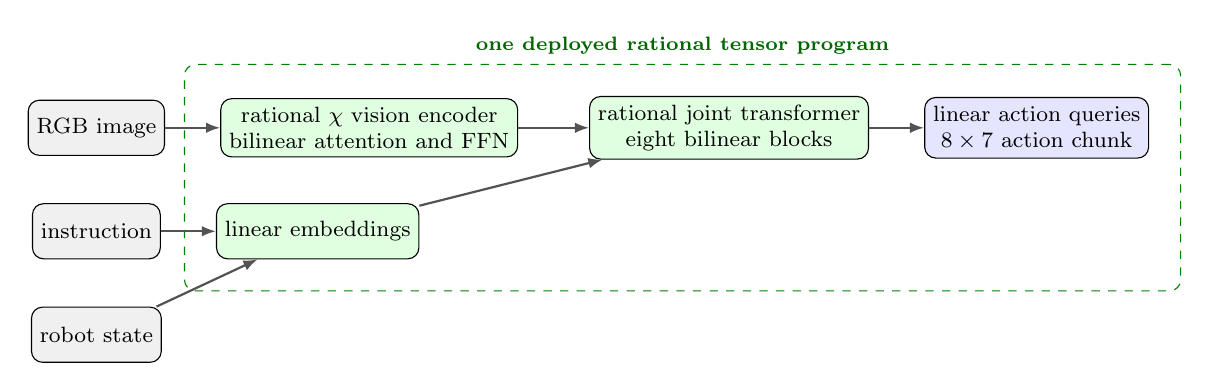
\begin{tikzpicture}[
  font=\footnotesize,
  box/.style={draw,rounded corners,align=center,minimum height=7mm,inner sep=3pt},
  inp/.style={box,fill=gray!12},
  prim/.style={box,fill=green!12},
  output/.style={box,fill=blue!10},
  arr/.style={-{Latex[length=1.8mm]},thick,gray!65!black},
  node distance=6mm and 7mm,
]
\node[inp] (img) {RGB image};
\node[inp, below=of img] (txt) {instruction};
\node[inp, below=of txt] (state) {robot state};
\node[prim, right=of img] (vision) {rational $\chi$ vision encoder\\bilinear attention and FFN};
\node[prim, right=of txt] (embed) {linear embeddings};
\node[prim, right=9mm of vision, minimum width=34mm] (joint) {rational joint transformer\\eight bilinear blocks};
\node[output, right=of joint] (action) {linear action queries\\$8\times7$ action chunk};
\draw[arr] (img) -- (vision);
\draw[arr] (txt) -- (embed);
\draw[arr] (state) -- (embed);
\draw[arr] (vision) -- (joint);
\draw[arr] (embed) -- (joint);
\draw[arr] (joint) -- (action);
\begin{scope}[on background layer]
\node[draw=green!50!black,dashed,rounded corners,fit=(vision)(embed)(joint)(action),
      inner sep=4mm,label={[green!40!black,font=\scriptsize\bfseries]above:one deployed rational tensor program}] {};
\end{scope}
\end{tikzpicture}}
\caption{\textbf{Deployed \chivla\ map.} The strongest checkpoints use one vision stream and a
linear continuous-action head. Every learned component inside the dashed boundary is linear,
bilinear, or rational.}
\label{fig:architecture}
\end{figure}

\subsection{Architecture and training}

The policy follows the high-level VLA sequence of visual encoding, language and state
embedding, joint processing, and action decoding \cite{openvla}. It uses a $64\times64$
agent-view image, an eight-dimensional robot state, a 26-token task vocabulary, and eight
action-query tokens. The joint backbone has width $384$, eight blocks, and twelve heads.
The action head maps each action-query state directly to seven continuous action dimensions.
The complete model has $20{,}137{,}352$ learned parameters.

Training uses $66{,}984$ demonstration frames, $40{,}000$ AdamW updates, batch size $256$,
cosine decay, bfloat16 arithmetic, and an exponential moving average. Closed-loop evaluation
uses a $180^\circ$ camera rotation to match the demonstration convention, canonical LIBERO
initial states, and fail-loud checks that verify every requested state was loaded.

\subsection{Mechanical certificate on the trained checkpoint}

Architecture definitions can differ from deployed code. We therefore audit the real
$189/200$ checkpoint at runtime and reconstruct representative operations from saved weights.

\begin{figure}[H]
\centering
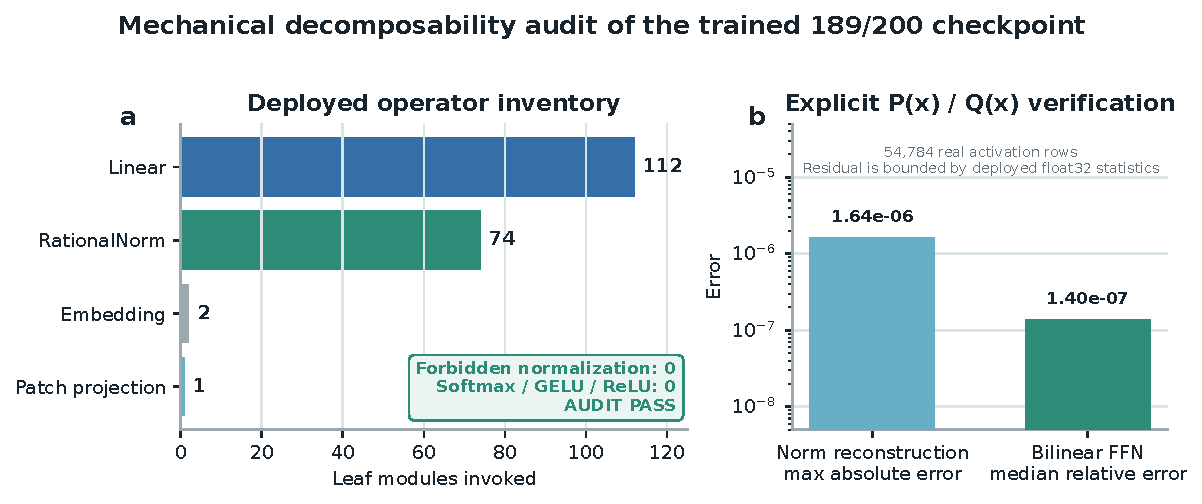
\includegraphics[width=0.88\textwidth]{../paper_figures/appendix_decomposability_audit.pdf}
\caption{\textbf{Mechanical audit of the trained rational checkpoint.} The runtime path invokes
$112$ linear maps, $74$ rational normalizers, two embeddings, and one linear patch projection.
No softmax, standard activation, or ordinary normalization is present. Reconstruction errors
are measured over $54{,}784$ real activation rows.}
\label{fig:audit}
\end{figure}

The normalization reconstruction has maximum absolute error $1.64\times10^{-6}$. A bilinear
FFN reconstruction has median relative error $1.40\times10^{-7}$. These residuals are bounded
by the deployed module's float32 statistic. The audit certifies operator membership and local
reconstruction. It does not materialize one compact polynomial for the full eight-layer
transformer.

% ============================================================================
\section{Protocol-aligned closed-loop capability}
\label{sec:capability}
% ============================================================================

\subsection{Evaluation protocol}

We evaluate all ten LIBERO-Object tasks with:

\begin{itemize}
  \item $50$ canonical trials per task
  \item a $280$-step cap
  \item three independently trained seeds per architecture
  \item $500$ rollouts per seed and $1{,}500$ rollouts per architecture
\end{itemize}

Published OpenVLA and Diffusion Policy results are protocol-aligned references. They were not
rerun in our codebase, so differences may still include implementation and training choices.

\begin{figure}[H]
\centering
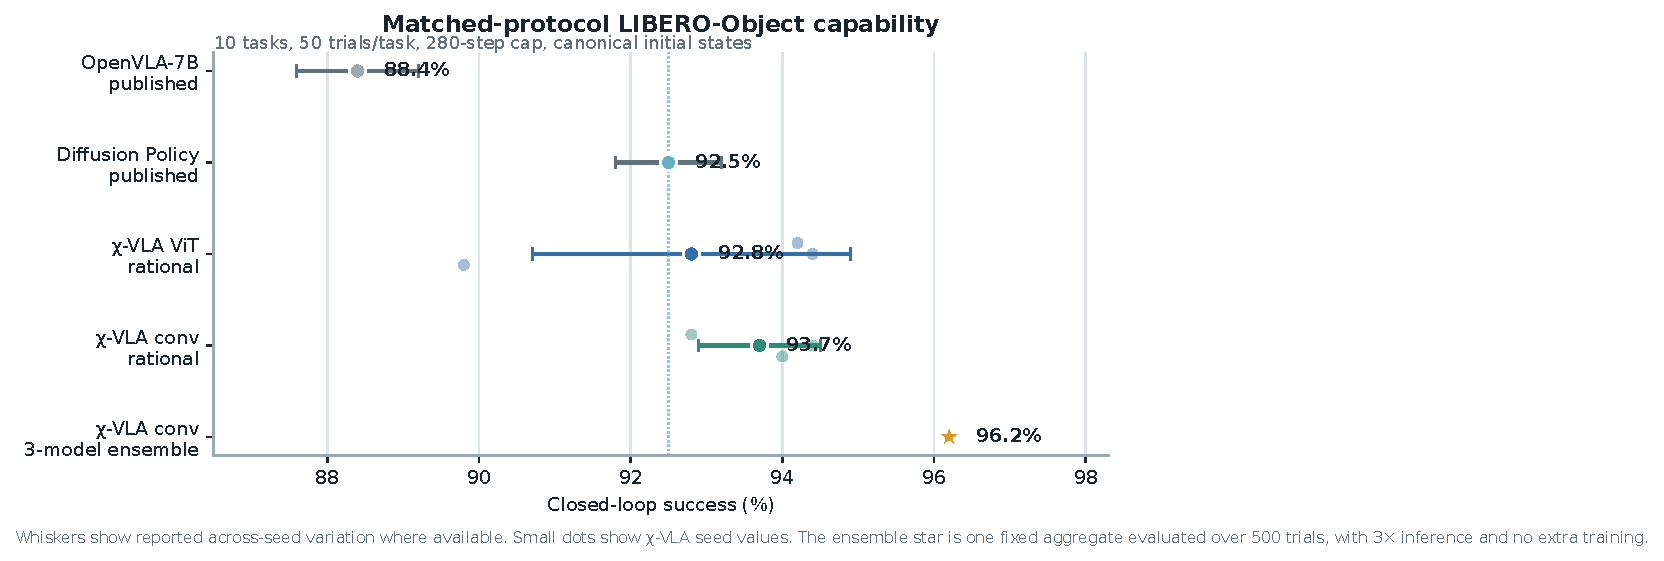
\includegraphics[width=0.92\textwidth]{../paper_figures/main_capability.pdf}
\caption{\textbf{Protocol-aligned LIBERO-Object capability.} Small dots are \chivla\ training
seeds. The ensemble star averages three convolutional checkpoints and uses three forward
passes per action chunk. External references are reported published values.}
\label{fig:capability}
\end{figure}

\subsection{Results}

\begin{table}[H]
\centering
\small
\begin{tabular}{@{}lccc@{}}
\toprule
Method & Parameters & Training seeds & Success \\
\midrule
\chivla, rational ViT & $20.1$M & $3$ & $92.8\%\pm2.1\%$ \\
Same-skeleton conventional ViT & $20.1$M & $1$ & $89.8\%$ \\
\chivla, rational conv & $20.1$M & $3$ & $\mathbf{93.7\%\pm0.8\%}$ \\
\chivla, conv ensemble & $3\times20.1$M & $3\to1$ & $\mathbf{96.2\%}$ \\
OpenVLA-7B \cite{openvla} & $7$B & $3$ & $88.4\%\pm0.8\%$ \\
Diffusion Policy \cite{openvla} & not matched & $3$ & $92.5\%\pm0.7\%$ \\
\bottomrule
\end{tabular}
\caption{\textbf{Closed-loop success under aligned evaluation settings.} The two external rows
are historical references rather than current state-of-the-art claims.}
\label{tab:capability}
\end{table}

The ViT seeds score $89.8\%$, $94.4\%$, and $94.2\%$. The convolutional seeds score
$94.0\%$, $94.4\%$, and $92.8\%$. The convolutional model is modestly higher and more
consistent in this three-seed comparison.

The same-skeleton conventional control replaces bilinear attention, bilinear FFNs, and rational
normalization with softmax attention, SwiGLU, and RMSNorm. It keeps the observations, token
layout, demonstrations, optimizer, updates, seed, action decoder, canonical initial states, and
trial budget fixed. In the initial Athena pass, the conventional policy succeeds in $449/500$
trials and the rational policy in $426/500$. The rational model has
$20{,}137{,}352$ parameters and the conventional model has $20{,}138{,}632$, a difference of
$0.006\%$. The pass assigns different task groups to A6000 and A30 hardware, and the sign of the
architecture difference changes between those groups. We therefore report it as a portability
warning rather than a clean capability-cost estimate. On one A30, eager batch-one latency is
$38.05$ ms for the rational model and $7.14$ ms for the conventional control. Compilation reduces
these to $1.52$ and $0.88$ ms, a $1.74\times$ gap. At batch $128$, rational training is
$3.12\times$ slower and uses $1.63\times$ the peak allocated memory.

Elementwise averaging of the three convolutional action predictions reaches $96.2\%$. This is
$2.3$ points above the mean of its members and $1.2$ points above the strongest member.
The gain is largest on tomato sauce, butter, and ketchup. The ensemble requires three complete
forward passes and is not one $20.1$M-parameter policy.

\subsection{What this result does and does not establish}

The result shows that the rational architecture supports high closed-loop specialist
capability and closes the first same-seed capability-cost comparison. One conventional seed is
not enough for a three-seed noninferiority claim, and the eager latency gap is material.
Additional conventional seeds, partial-conversion controls, and optimized execution are still
required before claiming that convertibility is broadly or computationally free.

% ============================================================================
\section{Exact weight-derived structure through attention}
\label{sec:exactattention}
% ============================================================================

\subsection{Exact layerwise construction}

Equation~\ref{eq:attention} contains two query-key products and one value stream. Expanding
the linear maps gives a high-order coefficient table. Each entry says how strongly one
combination of query, key, and value coordinates contributes to an output. It is
\emph{weight-derived} because no examples or fitted probe are needed to construct it. On a
tiny four-token, width-four, one-head layer, direct evaluation
and an independent explicit polynomial agree to $2.00\times10^{-15}$. The internal core
identity agrees to $1.24\times10^{-14}$.

The deployed attention also normalizes each query and key with Equation~\ref{eq:rnorm}.
Each normalization multiplies all channels of one token by the same scalar rational factor.
Those factors can be pulled outside the bilinear dot products. The polynomial attention core
is unchanged, while explicit numerator and denominator factors carry the normalization.
The rational extension agrees to $3.61\times10^{-16}$. We then reconstruct all four vision and
eight joint attention modules in each of three trained checkpoints, covering $384$ heads in
total. The worst relative $\ell_2$ error is $2.56\times10^{-7}$ and the worst absolute difference
is $2.23\times10^{-5}$. This residual comes from the deployed implementation's intentional
float32 statistic, while the reconstruction itself uses the learned coefficients.

Naively materializing the real width-$384$ coefficient tensor would require approximately
$3.2\times10^{15}$ values. We instead contract the CP factors into an $O(d^2)$ reduced Gram.
This smaller matrix plays the role of a covariance matrix: its leading eigenvectors rank the
directions that carry the most coefficient energy without constructing the full table. At toy
multi-head scale, it matches brute-force materialization to $2.13\times10^{-14}$.

\subsection{Trained policy result}

For the subspace-ranking experiment, we apply the exact weight-derived calculation to all twelve
heads in early, middle-late, and
final backbone blocks $0$, $6$, and $7$. Random projector banks are sampled once, then fixed
and reused for all evaluation examples. The weights choose the subspace. Real cached
activations are used only afterward to measure how faithfully that subspace preserves the
layer's computation.

\begin{figure}[H]
\centering
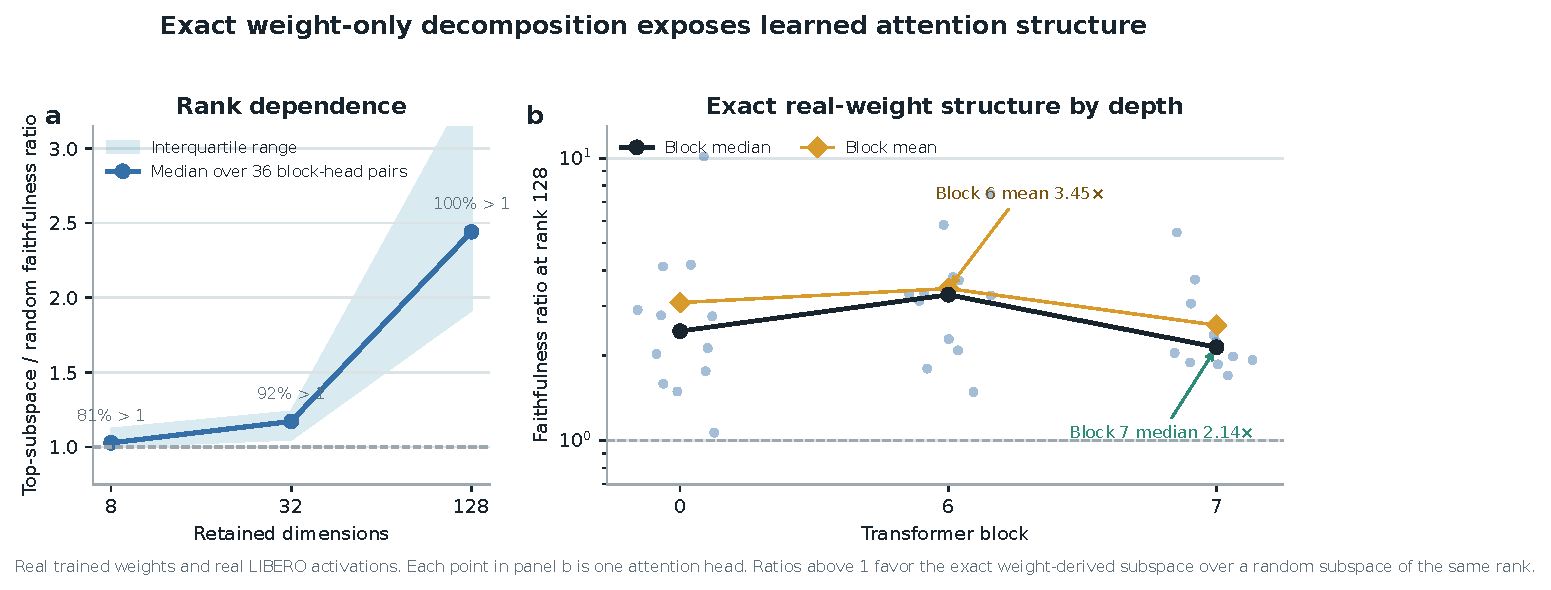
\includegraphics[width=0.94\textwidth]{../paper_figures/main_exact_attention_odt.pdf}
\caption{\textbf{Exact weight-derived attention structure.} Ratios above one favor the exact
weight-derived subspace over a random equal-rank subspace. Each point in the right panel is one
trained attention head.}
\label{fig:exactattention}
\end{figure}

At ranks $8$, $32$, and $128$, respectively, $80.6\%$, $91.7\%$, and $100\%$ of the $36$
block-head pairs favor the exact subspace. Their median ratios are $1.028$, $1.171$, and
$2.441$. At rank $128$, the mean ratio is $3.033$ and the strongest head reaches $10.135$.
The rank-$128$ block means are $3.08$, $3.45$, and $2.56$ for blocks $0$, $6$, and $7$.

This extends exact weight-only construction through individual attention layers. It is not an
exact end-to-end decomposition of the complete policy. Composition across all eight blocks
still faces rapid degree and representation growth.

% ============================================================================
\section{Causal policy structure and a language shortcut}
\label{sec:causal}
% ============================================================================

We next test whether the identified structure affects closed-loop behavior and whether high
task success reflects robust use of the language input.

\subsection{Causal visual subspace}

At the visual bond before the joint backbone, we rank directions separately for translation,
rotation, and gripper actions. A subspace is a smaller coordinate system inside the model's
$384$-dimensional visual representation. Retaining a subspace means zeroing every direction
outside it, then running the actual policy. We compare the selected directions with random
equal-width controls in offline reconstruction and closed-loop intervention. This ranking uses
held-out activations and downstream sensitivity, so it tests a causal bottleneck but is not a
weight-only discovery result.

\begin{figure}[H]
\centering
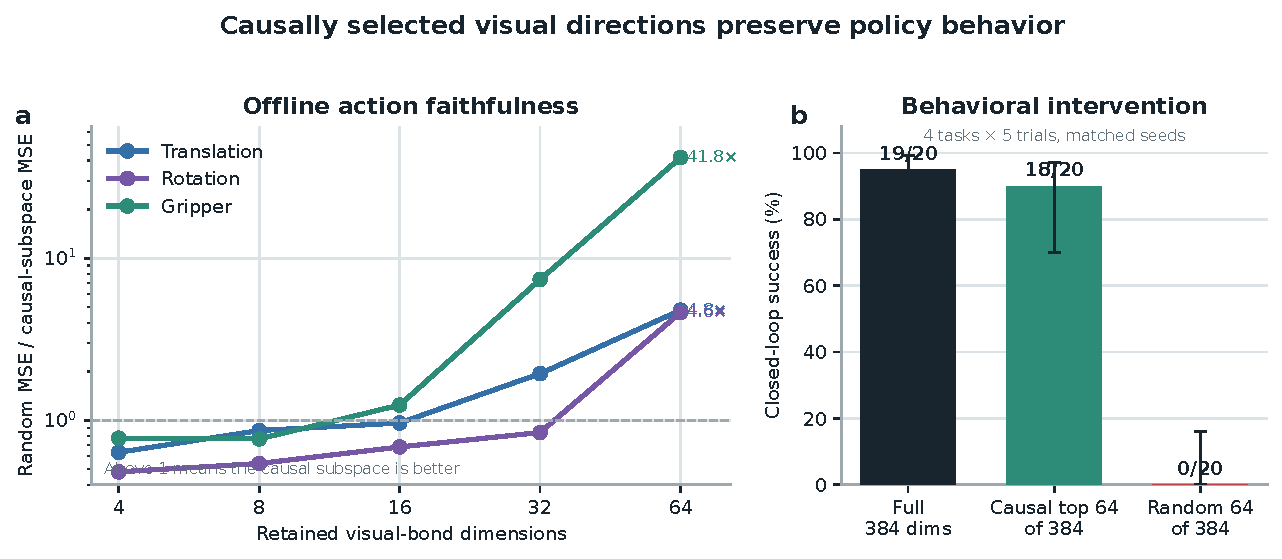
\includegraphics[width=0.94\textwidth]{../paper_figures/main_causal_subspace.pdf}
\caption{\textbf{Causally selected visual directions preserve policy behavior.} The left panel
reports random MSE divided by selected-subspace MSE. The right panel intervenes on the real
policy over four tasks and five paired trials per task.}
\label{fig:causal}
\end{figure}

With $64$ of $384$ dimensions retained, the selected subspace reduces action reconstruction
error relative to random by $4.8\times$ for translation, $4.6\times$ for rotation, and
$41.8\times$ for the gripper. In closed loop, the full representation succeeds in $19/20$
trials, the selected subspace in $18/20$, and a random subspace in $0/20$.

This result establishes a causal low-dimensional substrate, but it is still limited to one
checkpoint and twenty rollouts. The current ranking at this full-policy bond uses held-out
examples and downstream sensitivity. The exact layerwise attention method in
Section~\ref{sec:exactattention} must still be connected to the same full-suite closed-loop
intervention.

\subsection{Counterfactual instruction test}

High success does not guarantee robust language use. A one-step screen is weak: replacing the
instruction with one naming another visible object shifts the predicted reach direction toward
that object in only $15.0\%$ of $80$ canonical states. We therefore run paired $80$-step
rollouts from $100$ matched canonical states for each of three checkpoints. The instruction
change increases relative end-effector preference for the renamed object by $0.175$, $0.168$,
and $0.189$ m. All three trial-bootstrap $95\%$ intervals exclude zero. The trajectories shift
toward the renamed object in $84\%$, $86\%$, and $88\%$ of pairs, but end closer to it in only
$33\%$, $28\%$, and $28\%$. Appendix Figure~\ref{fig:counterfactual-grounding} reports the
replication. The seed-0 conventional twin responds even more strongly, with a $0.239$ m shift,
$92\%$ directional response, and a $33\%$ endpoint rate. Instruction responsiveness is therefore
not unique to the algebraic architecture. This is behavioral grounding evidence, not
counterfactual task success, because
the benchmark predicate still names the original object and the horizon covers the reach phase.

The likely shortcut is structural in the dataset. Each scene template is paired with an almost
fixed target, so scene identity can substitute for object-name grounding. Decorrelated
scripted demonstrations improve the counterfactual metric, but all three fine-tuning attempts
severely reduce ordinary closed-loop success. The best repaired dataset raises capability only
to $21.5\%$, far below the healthy range.

This mixed result narrows the VLA claim. Language changes the trajectory reproducibly, but scene
priors often prevent complete rerouting. The model is therefore a capable language-conditioned
specialist, not yet a robust instruction-grounded policy. LIBERO-CF independently
documents the same broad failure class in existing VLAs \cite{liberocf}. Our prospective
novelty is therefore not the shortcut alone. It is the harder test of whether exact
weight-derived terms can localize and selectively repair that shortcut.

% ============================================================================
\section{Decisive remaining tests}
\label{sec:next}
% ============================================================================

\paragraph{1. Complete the controlled conversion study.}
Finish the same-hardware seed-0 matrix, then complete seeds 1 and 2, add partial-conversion
controls, and retain the predeclared three-point noninferiority margin.
Report FLOPs, training throughput, memory, eager latency, and optimized latency separately.
The current evidence supports strong rational capability, not a settled conversion-cost estimate.

\paragraph{2. Direct coefficient surgery.}
Our first preregistered four-task screen directly edits query, key, and value columns selected
by exact attention Grams. Retention gives a favorable $10$-point gap over random controls but
misses the $15$-point gate, while removal has the wrong sign. This is a no-go for the current
edit mapping, as detailed in Appendix~\ref{app:expanded-mechanisms}. The next test must resolve
redundant paths or gauge sensitivity, compare post-hoc controls across three checkpoints, and
report targeted effect, ordinary success, edit norm, and collateral damage.

\paragraph{3. Concrete diagnosis and selective repair.}
Develop two capstones. Gripper timing is the lower-risk target because phase transitions and
premature closure have explicit simulator variables. Scene identity versus instruction
binding is the higher-upside target because the current policy demonstrably fails the
counterfactual test. In both cases, discover the algebraic term from weights, attach a limited
semantic label, freeze the candidate, predict the behavioral consequence, and test on blind
paired rollouts. A compelling repair should improve the targeted failure by $10$ to $20$
points, lose no more than $2$ to $3$ points of ordinary success, and preserve its direction
across three seeds.

\paragraph{4. Broader capability and grounding.}
Evaluate the conventional and rational finalists on LIBERO-Goal and LIBERO-Long, followed by a
counterfactual grounding benchmark such as LIBERO-CF \cite{liberocf}. Object-only success is
insufficient because standard LIBERO can reward scene-to-action memorization \cite{liberopro}.
Test the stability of recovered mechanisms under equivalent reparameterizations and across
trained seeds.

\paragraph{5. RL only after a paired gate.}
The repaired-reward AWR pilot improves $80.7\%$ to $82.7\%$, but it has one seed and fifteen
trials per task. A justified follow-up needs three paired seeds, a matched-compute
behavior-cloning continuation control, full protocol evaluation, and regression gates.
Generic PPO on saturated LIBERO-Object is lower priority than the four tests above.

% ============================================================================
\section{Related work}
% ============================================================================

\paragraph{VLA capability.}
OpenVLA established an open pretrained VLA and standardized LIBERO comparisons
\cite{openvla}. OpenVLA-OFT showed that continuous action chunks and simple regression can
substantially improve adaptation and control efficiency \cite{openvlaoft}. These systems use
large pretrained backbones. \chivla\ instead studies a compact from-scratch specialist under
an algebraic restriction.

\paragraph{Tensor and polynomial networks.}
Polynomial networks and tensor networks use explicit multilinear structure for representation
and learning \cite{koldabader,stoudenmire,chrysos}. Bilinear MLP work showed that weight
eigendecomposition can expose low-rank features and circuits \cite{pearce}. $\chi$-nets
introduced ODT for compositional bilinear networks \cite{chinets}. We extend the setting to a
continuous closed-loop policy and give an exact reduced construction for individual
softmax-free attention layers.

\paragraph{Causal mechanisms and policy analysis.}
Bilinear IMPALA policies have combined competitive ProcGen control with weight-derived
eigenfilters, followed by activation probing and control \cite{bimpala}. This is the closest
architectural precedent for weight-based policy analysis. Recent work steers pretrained VLAs
through causally identified activation directions \cite{haonsteering}. Sparse feature circuits identify and
edit causal feature graphs in conventional language models \cite{sparsecircuits}, while
nonlinear causal reductions recover behavioral patterns in reinforcement-learning policies
from rollout perturbations \cite{causalreduction}. These results make a universal separation
from conventional policies untenable. Our intended distinction is empirical: exact
weight-derived discovery and direct coefficient edits in a competitive continuous
vision-language policy, evaluated for stability and collateral damage against matched
post-hoc baselines.

\paragraph{VLA robustness.}
Recent evaluations show that standard LIBERO success can coexist with weak robustness and
language use \cite{liberopro,liberocf,liberopara}. Our instruction intervention reaches the
same conclusion from an independently trained compact specialist and motivates a
decomposition-guided diagnosis.

% ============================================================================
\section{Limitations and conclusion}
% ============================================================================

\chivla\ demonstrates that a complete rational tensor policy can reach strong specialist
closed-loop capability. The real checkpoint passes a mechanical operator audit. Exact
weight-derived analysis now crosses individual attention layers, and a compact causal visual
subspace preserves almost all tested behavior.

Five limits determine the next version of the paper. First, the same-skeleton control has one
completed seed, a hardware-confounded capability comparison, and a residual compiled-runtime
tax. Second, the
benchmark is one narrow suite and counterfactual instructions do not fully reroute the policy.
Third, exact
decomposition is layerwise rather than end to end. Fourth, the closed-loop causal intervention
uses one checkpoint and twenty trials. Fifth, activation projection succeeds but the first
direct coefficient-edit screen fails its selectivity gate, so no behaviorally validated weight
edit has yet been established.

The defensible conclusion is therefore narrow. Polynomial and rational restrictions do not
prevent a compact policy from reaching competitive LIBERO-Object capability. The current
matched control does not yet isolate architecture from device sensitivity. The restrictions
also provide a precise
weight-derived analysis surface. Establishing multi-seed conversion cost, broad
language-grounded control, semantic diagnosis from weights, and a decomposition-enabled repair
requires the controlled experiments in Section~\ref{sec:next}. If all three conjuncts in
Table~\ref{tab:thesis} hold on the same trained policies, the result is stronger than any
individual capability, decomposition, or intervention claim.

\paragraph{Reproducibility.}
Training and evaluation use fixed task lists, explicit camera and action conventions,
canonical-state manifests, checkpointed moving-average weights, and per-run result files.
The final artifact will release code, checkpoint hashes, exact attention certificates, and
per-episode evaluation logs. Preflight checks fail if canonical initial states cannot be
loaded.

% ============================================================================
\begin{thebibliography}{99}

\bibitem{openvla}
M.~J. Kim et al.
\newblock \emph{OpenVLA: An Open-Source Vision-Language-Action Model.}
\newblock CoRL, 2024.

\bibitem{openvlaoft}
M.~J. Kim, C.~Finn, and P.~Liang.
\newblock \emph{Fine-Tuning Vision-Language-Action Models: Optimizing Speed and Success.}
\newblock 2025.

\bibitem{pearce}
A.~Rigg, T.~Dooms, M.~T. Pearce, J.~Oramas, and L.~Sharkey.
\newblock \emph{Bilinear MLPs Enable Weight-Based Mechanistic Interpretability.}
\newblock ICLR, 2025.

\bibitem{chinets}
T.~Dooms, W.~Gauderis, G.~A. Wiggins, and J.~Oramas.
\newblock \emph{Compositionality Unlocks Deep Interpretable Models.}
\newblock 2025.

\bibitem{bimpala}
F.~Oozeer, Y.~Erisken, A.~Rigg, J.~Oramas, and L.~Sharkey.
\newblock \emph{Bilinear Convolution Decomposition for Causal RL Interpretability.}
\newblock 2024.

\bibitem{haonsteering}
B.~H\"aon, K.~Stocking, I.~Chuang, and C.~Tomlin.
\newblock \emph{Mechanistic Interpretability for Steering Vision-Language-Action Models.}
\newblock 2025.

\bibitem{sparsecircuits}
S.~Marks et al.
\newblock \emph{Sparse Feature Circuits: Discovering and Editing Interpretable Causal Graphs
in Language Models.}
\newblock ICLR, 2025.

\bibitem{causalreduction}
M.~Keki\'c et al.
\newblock \emph{Learning Nonlinear Causal Reductions to Explain Reinforcement Learning
Policies.}
\newblock ICLR, 2026.

\bibitem{liberopro}
X.~Zhou et al.
\newblock \emph{LIBERO-PRO: Towards Robust and Fair Evaluation of Vision-Language-Action
Models Beyond Memorization.}
\newblock 2025.

\bibitem{liberocf}
Y.~Fang et al.
\newblock \emph{When Vision Overrides Language: Evaluating and Mitigating Counterfactual
Failures in VLAs.}
\newblock 2026.

\bibitem{liberopara}
C.~Kim et al.
\newblock \emph{LIBERO-Para: A Diagnostic Benchmark and Metrics for Paraphrase Robustness in
VLA Models.}
\newblock 2026.

\bibitem{koldabader}
T.~Kolda and B.~Bader.
\newblock \emph{Tensor Decompositions and Applications.}
\newblock SIAM Review, 2009.

\bibitem{stoudenmire}
E.~Stoudenmire and D.~Schwab.
\newblock \emph{Supervised Learning with Tensor Networks.}
\newblock NeurIPS, 2016.

\bibitem{chrysos}
G.~Chrysos et al.
\newblock \emph{Deep Polynomial Neural Networks.}
\newblock CVPR and TPAMI, 2020 to 2021.

\end{thebibliography}

% ============================================================================
\appendix
\section{Supporting results and decisions}
% ============================================================================

\subsection{Original 94.5\% capability result}

Before the final protocol-aligned benchmark, one rational ViT checkpoint succeeded in
$189/200$ trials under a $600$-step horizon and $20$ trials per task. This result established
that the rational implementation could support all ten tasks. It should not be compared
directly with the protocol-aligned external references because it uses one training seed, fewer
trials, and a longer horizon.

\subsection{Matched architecture capability and systems cost}

\begin{figure}[H]
\centering
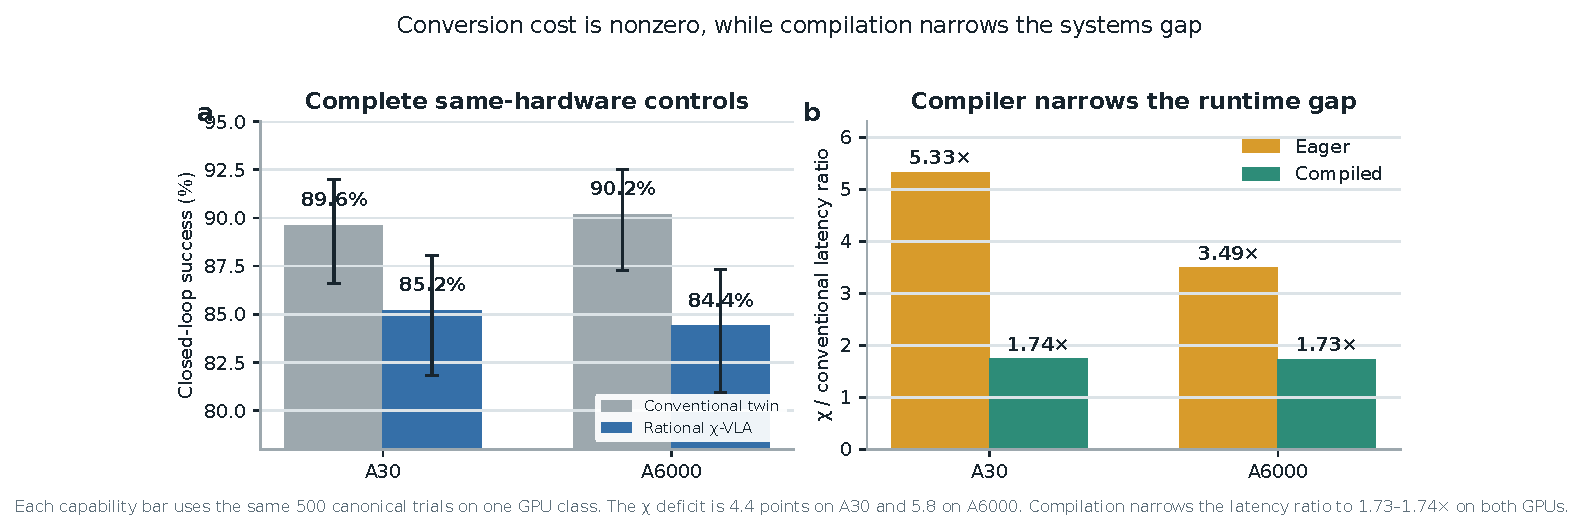
\includegraphics[width=0.96\textwidth]{../paper_figures/appendix_matched_architecture_cost.pdf}
\caption{\textbf{The initial capability pass is hardware-confounded, while the systems control
is not.} The mixed-device evaluation gives $449/500$ conventional and $426/500$ rational
successes, with a $0.006\%$ parameter difference. On the same A30, compilation narrows the
batch-one latency ratio from $5.33\times$ to $1.74\times$.}
\label{fig:matched-cost}
\end{figure}

\subsection{Three-checkpoint counterfactual grounding}

\begin{figure}[H]
\centering
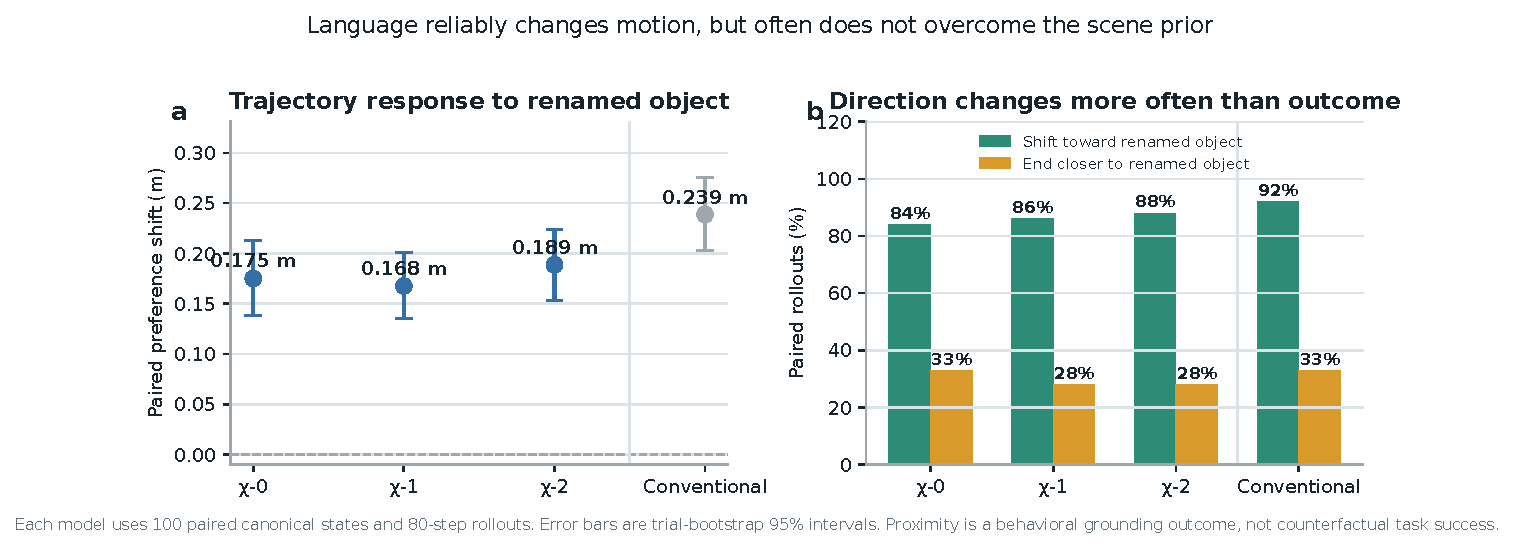
\includegraphics[width=0.96\textwidth]{../paper_figures/appendix_counterfactual_grounding.pdf}
\caption{\textbf{Renaming the target changes motion reliably but does not fully override the
scene prior.} Each model is evaluated on $100$ paired canonical states for $80$ control
steps. The left panel reports the change in end-effector preference for the newly named object,
with $95\%$ bootstrap intervals. The right panel separates directional response from the
stricter condition of ending closer to that object. These are proximity tests, not
counterfactual task-success measurements. The conventional control shows that ordinary language
response is not unique to tensor decomposability.}
\label{fig:counterfactual-grounding}
\end{figure}

\subsection{Per-task ensemble behavior}

\begin{figure}[H]
\centering
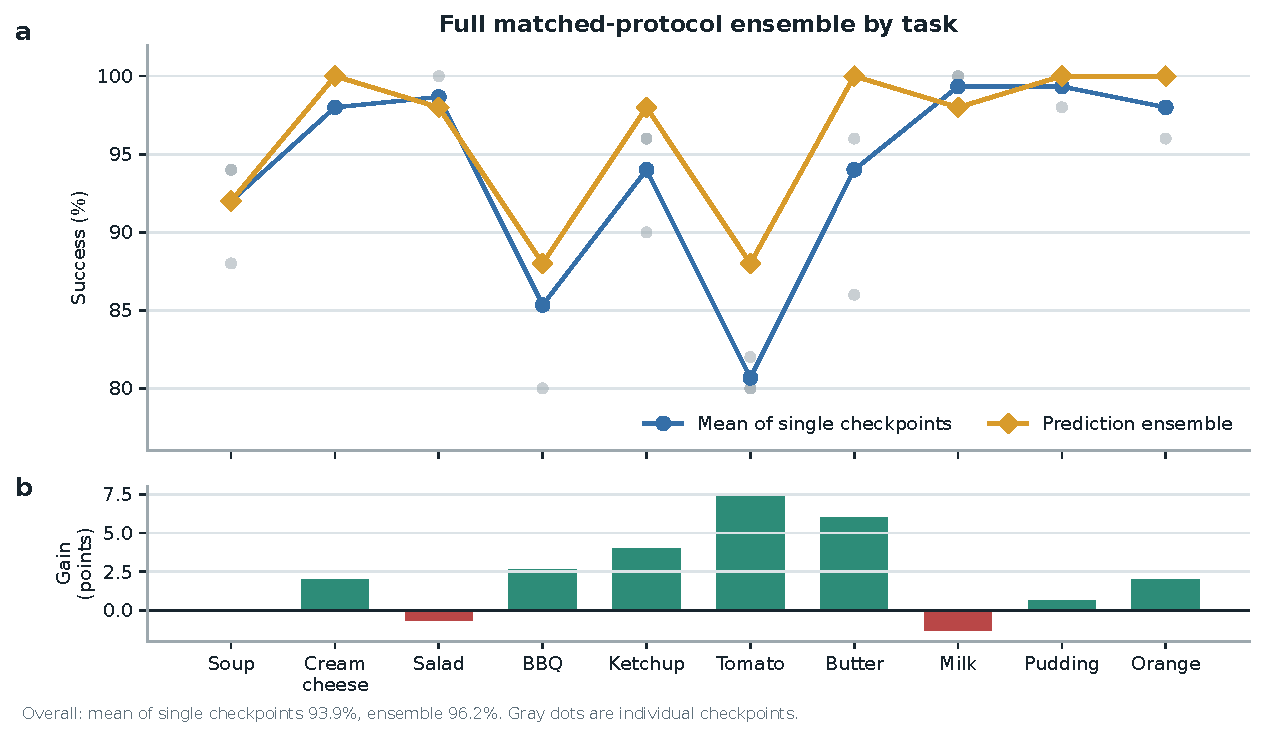
\includegraphics[width=0.96\textwidth]{../paper_figures/appendix_ensemble_per_task.pdf}
\caption{\textbf{Per-task effect of prediction averaging.} Gray points are the three
convolutional checkpoints, evaluated with $50$ canonical trials per task. Curves compare their
taskwise mean with elementwise action-prediction averaging. The ensemble raises overall success
from a $93.9\%$ member mean to $96.2\%$, with its largest gains on tomato sauce, butter, and
ketchup. It requires three forward passes and is not a single $20.1$M-parameter policy.}
\label{fig:ensemble-task}
\end{figure}

\subsection{Product-routing multimodal head}

For an action-query state $h$, the product-routing head represents
\begin{equation}
a(h,b)=c_0(h)+\sum_{g=1}^{G}(2b_g-1)c_g(h),
\qquad b\in\{0,1\}^{G}.
\end{equation}
The center, offsets, and gates are bilinear CP modules. A final external sign choice selects
one of $2^G$ modes. The head folds to numerical precision, but its five-seed closed-loop mean
is $44\%\pm30\%$ and its range overlaps the linear baseline. The strongest rational policy
therefore uses the linear head. Product routing remains a construction result until it wins a
controlled genuinely multimodal task.

\subsection{Development interventions}

Focused DAgger on BBQ and tomato improves combined success from $82.5\%$ to $96.0\%$ using
seven corrective episodes and $1{,}131$ frames. Applying the same update thinly across all ten
tasks reduces overall success from $92.0\%$ to $72.0\%$. Three original AWR runs decline by
$8.0$, $4.6$, and $2.6$ points. A reward audit shows that accumulated step cost makes every
successful trajectory have negative return. After removing that term and repairing the
terminal boundary, one pilot improves by two points. These are development diagnostics, not
validated paper contributions.

\begin{figure}[H]
\centering
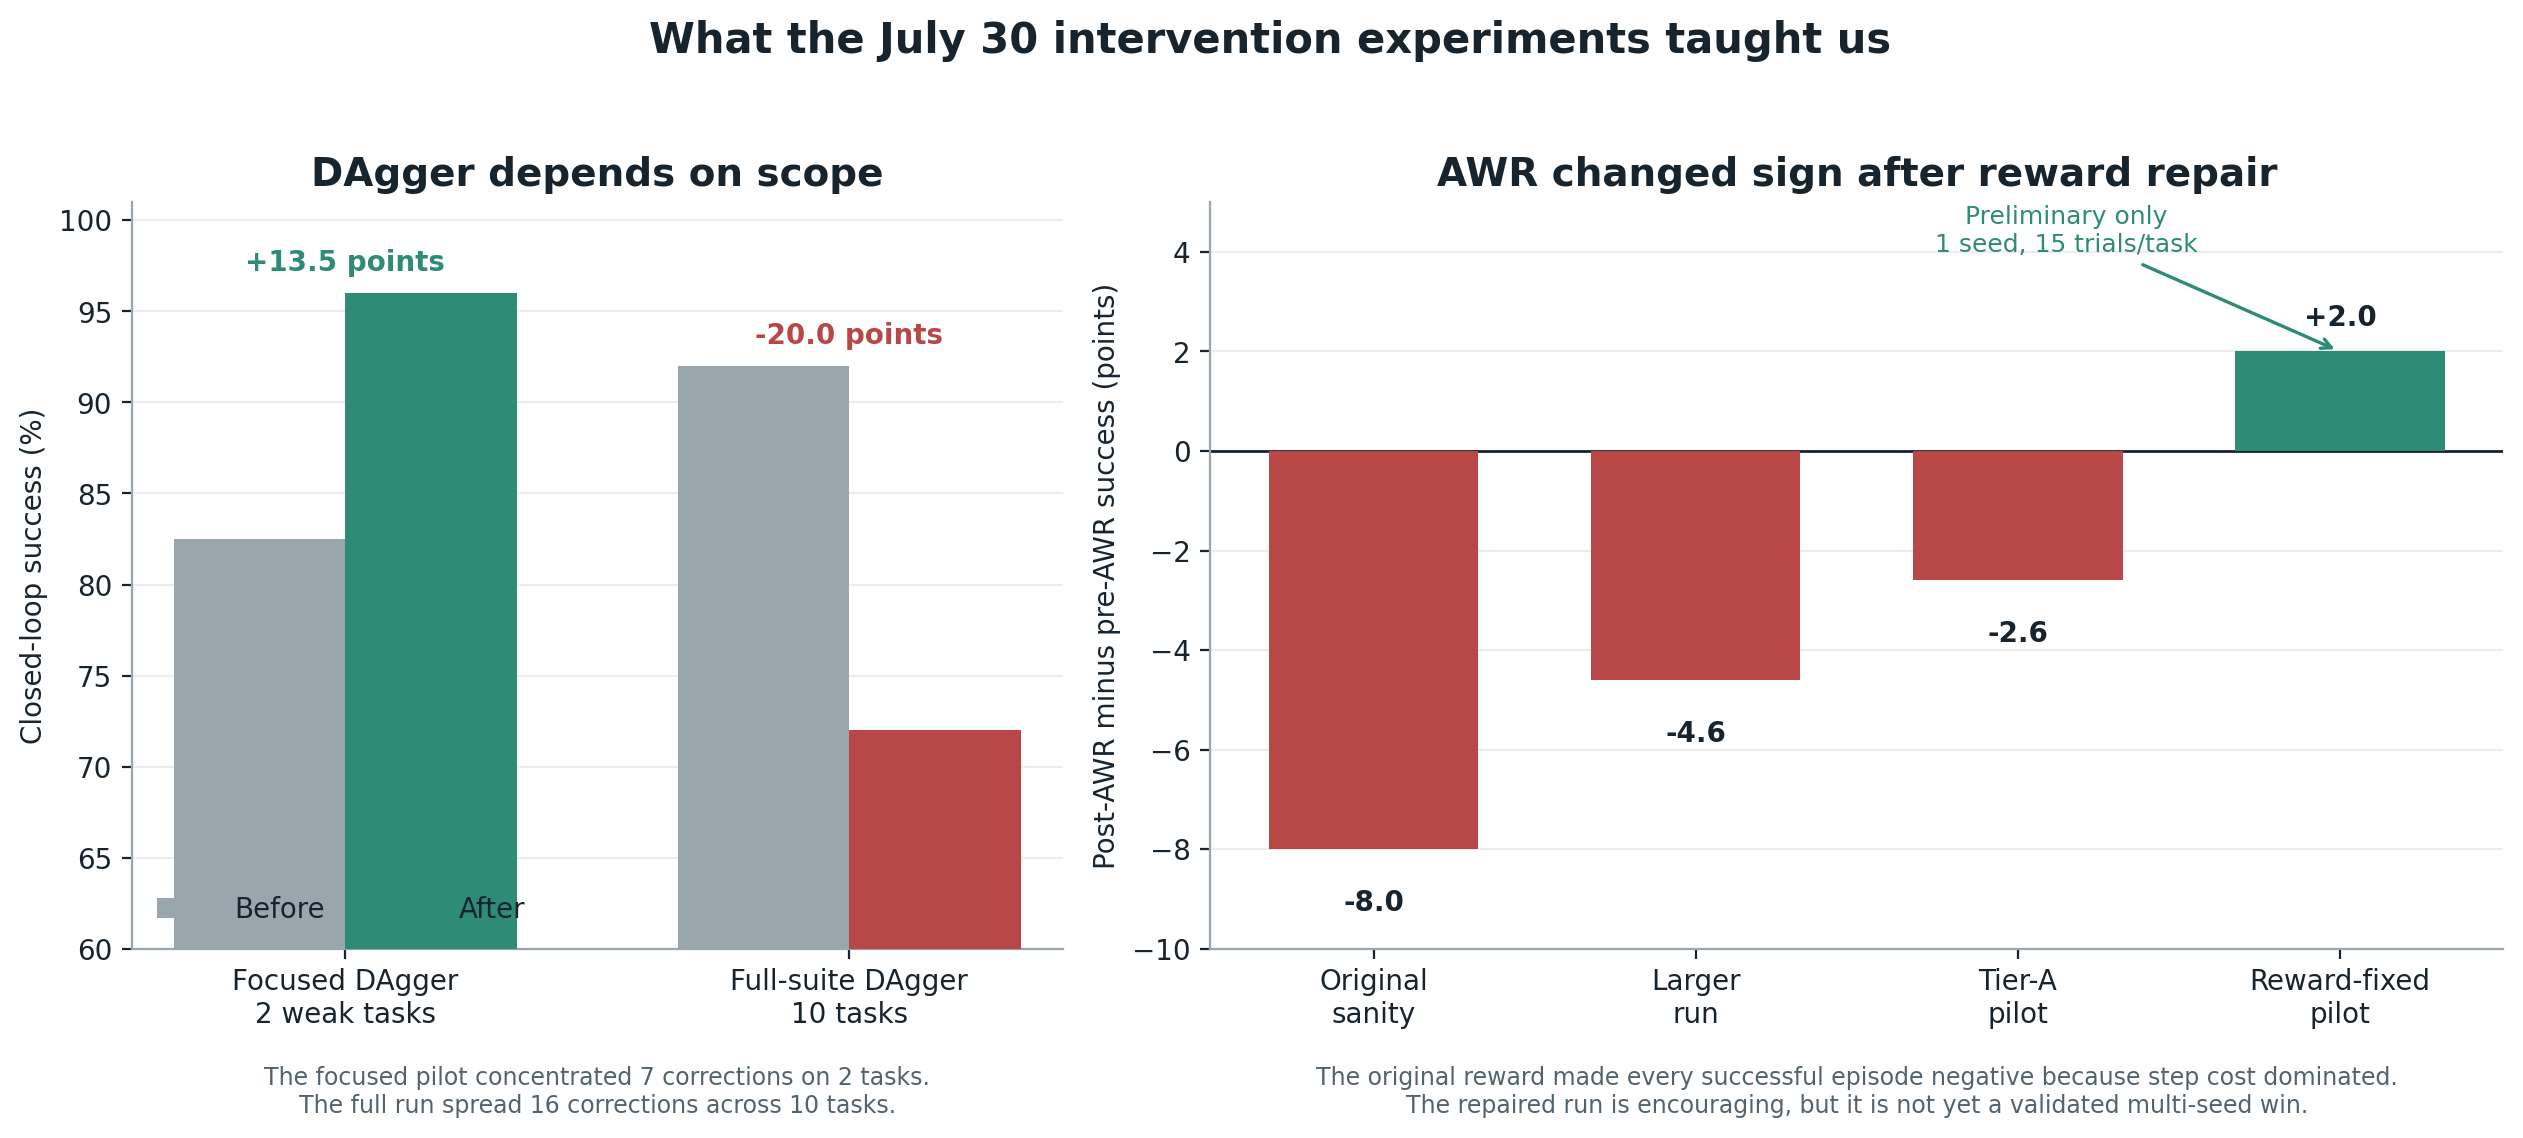
\includegraphics[width=0.98\textwidth]{../progress_figures/intervention_results.png}
\caption{\textbf{Development interventions reveal scope and reward sensitivity.} Focused
DAgger helps two weak tasks, while spreading a small correction budget across ten tasks causes
regression. Three AWR variants also regress before a reward audit and repair. The positive
reward-repaired AWR result is a one-seed pilot with $15$ trials per task, so it is not evidence
of a validated improvement.}
\label{fig:development-interventions}
\end{figure}

\subsection{Expanded attention screen and first direct edit}
\label{app:expanded-mechanisms}

The corrected fixed-control attention analysis covers all eight blocks and twelve heads. At
rank $128$, $83/96$ block-head pairs favor the exact weight-derived subspace. The median ratio
is $1.94$, the mean is $2.58$, and blocks $2$ and $3$ provide useful weak or negative controls.
At ranks $8$ and $32$, only $54/96$ and $60/96$ pairs favor the exact subspace. The effect is
therefore depth-dependent and strongest at the wider tested rank.

The first direct weight-edit screen uses four tasks and five paired canonical episodes per
task. Exact-subspace retention preserves $18/20$ successes compared with $16/20$ for both
random controls. This $10$-point advantage misses the preregistered $15$-point gate. Exact
removal also preserves $18/20$, compared with $17/20$ for both random controls, which is the
wrong direction for the necessity prediction. The screen is a no-go for the current mapping
from Gram eigenspaces to query, key, and value column edits.

\begin{figure}[H]
\centering
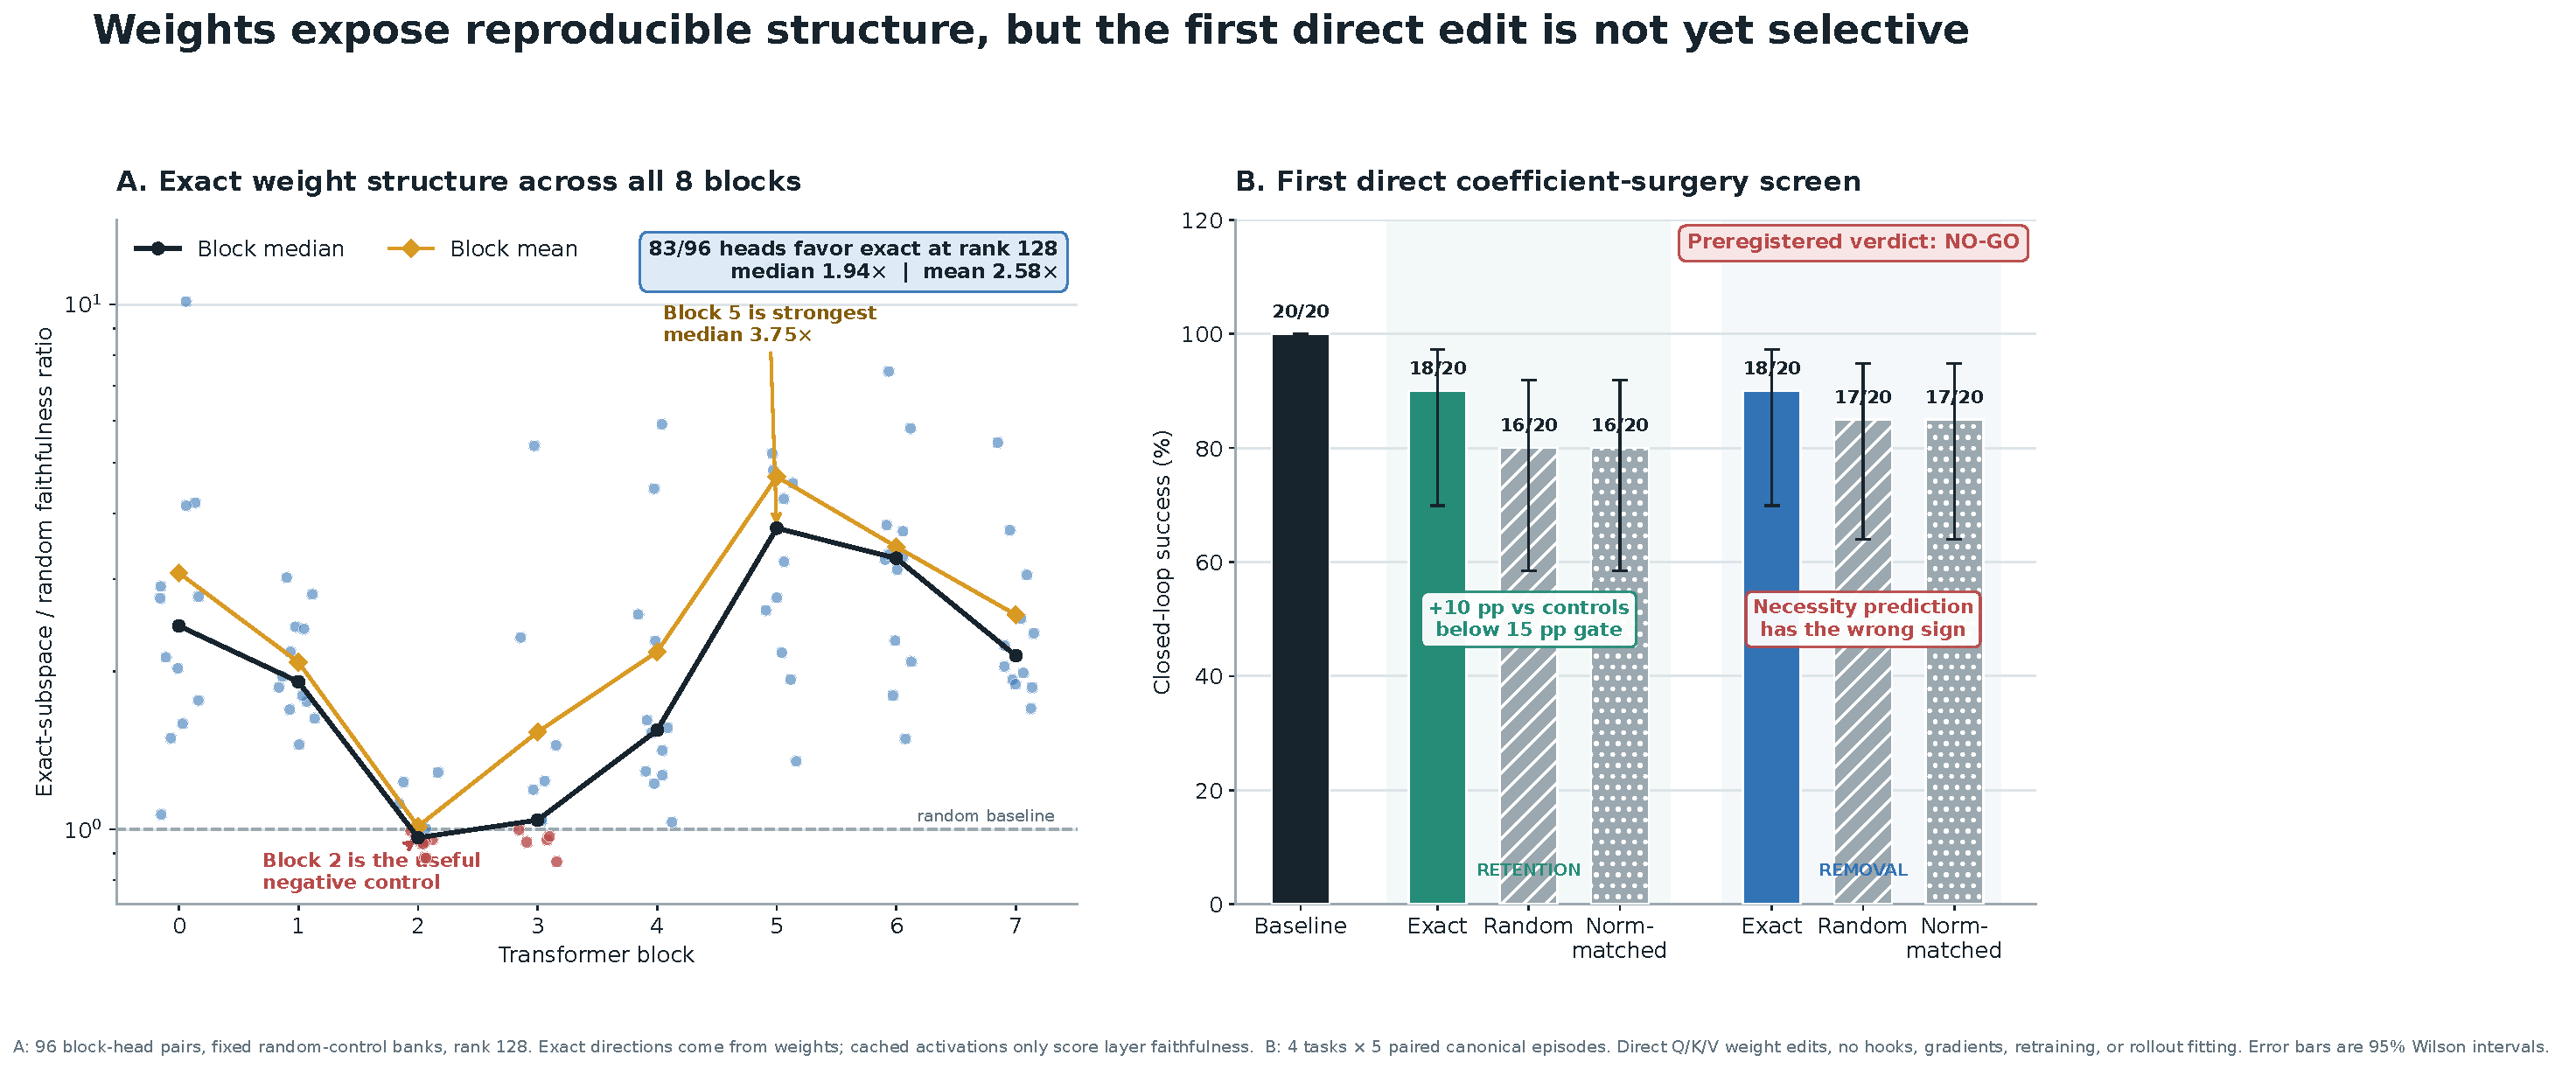
\includegraphics[width=0.98\textwidth]{../paper_figures/presentation_july31_mechanism_results.pdf}
\caption{\textbf{Expanded weight-structure and direct-surgery results.} Left: all $96$
block-head pairs at rank $128$, with fixed random-control banks. Exact directions come from
weights, while cached activations only score layer faithfulness. Right: the first direct
query-key-value column-edit screen over four tasks and five paired trials per task. Error bars
are $95\%$ Wilson intervals. The preregistered verdict is no-go because retention misses the
effect-size gate and removal has the wrong sign.}
\label{fig:expanded-mechanisms}
\end{figure}

\subsection{Numerical scope of rational conversion}

The deployed Pad\'e computation is exactly rational even though it approximates RMS
normalization. Final certification must report its polynomial degrees, coefficients,
denominator margin, observed activation range, tail error, action drift, and runtime overhead.
Operator membership alone does not establish practical numerical safety under distribution
shift.

\end{document}
